\documentclass[10pt,a4paper]{article}

\usepackage[margin=1.5cm]{geometry}
\usepackage{graphicx}
\graphicspath{{images/}}
\usepackage{multicol}
\usepackage{fancyhdr}
\usepackage{float}
\usepackage{listings}
\usepackage{xcolor}
\usepackage[T1]{fontenc}
\usepackage[utf8]{inputenc}
\usepackage{booktabs}
\usepackage{subcaption} % Required for side-by-side images
\usepackage{placeins}

\setlength{\columnsep}{0.6cm}

\pagestyle{fancy}
\fancyhf{}
\fancyfoot[R]{Page \thepage}
\renewcommand{\headrulewidth}{0pt}

\definecolor{codebackground}{RGB}{245,247,249}
\definecolor{codecomment}{RGB}{88,96,105}
\definecolor{codetag}{RGB}{0,92,153}
\definecolor{codestring}{RGB}{145,80,0}
\definecolor{codenumber}{RGB}{122,65,160}
\definecolor{codekeyword}{RGB}{128,32,96}
\lstdefinelanguage{XACRO}{
  language=XML,
  morekeywords={xacro:property,xacro:macro,xacro:include},
  tagstyle=\color{codetag}\bfseries,
  stringstyle=\color{codestring},
  numberstyle=\color{codenumber},
  keywordstyle=\color{codekeyword}\bfseries
}
\lstdefinelanguage{YAML}{
  morekeywords={ros_topic,gz_topic,ros_type,gz_type,direction},
  keywordstyle=\color{codekeyword}\bfseries
}
\lstset{
  basicstyle=\ttfamily\scriptsize,
  backgroundcolor=\color{codebackground},
  frame=single,
  rulecolor=\color{black!15},
  framerule=0.4pt,
  breaklines=true,
  columns=fullflexible,
  keepspaces=true,
  showstringspaces=false,
  commentstyle=\color{codecomment},
  keywordstyle=\color{codekeyword}\bfseries,
  stringstyle=\color{codestring},
  numberstyle=\color{codenumber},
  xleftmargin=0.2cm,
  xrightmargin=0.2cm
}

\begin{document}

\begin{center}
    {\LARGE \textbf{Assignment 3}}\\

    \vspace{0.15cm}

    {\Large \textbf{Applied Robotics and Autonomous Systems}}

    \vspace{0.3cm}

    ACIT4820-1 26H Oslomet

    \vspace{0.3cm}

    Nikolai Skaaheim-Grøna \\
    Lucas Van Der Horst \\
    Øyvind Amundsen Kjeang

    \vspace{0.3cm}

    Student numbers: 415337, 422009, oykje5980
\end{center}

\vspace{0.4cm}

\tableofcontents

\vspace{0.5cm}


\section{Introduction}

This report documents the modelling, verification, and control work completed for the robot platform in Assignment 3.

\section{Task 1: Finalise the Doomba's Body and Physics}

The provided Assignment 2 package was used as the starting point. The three provided \texttt{.dae} mesh files were downloaded and placed in the \texttt{meshes/} folder. The \texttt{<visual>} elements in \texttt{robot\_core.xacro} and \texttt{lidar.xacro} were updated to use meshes for the body, wheels and LiDAR. The collision geometry was kept unchanged, and the caster kept its sphere geometry. The mesh folder was included in \texttt{setup.py} so that the files were installed when the package was rebuilt.

\subsubsection*{Mesh Troubleshooting}

On the first day, several mesh components overlapped in RViz, as shown in Figure~\ref{fig:mesh_overlap_error}. The required geometry for each part was separated and converted to STL files. The Xacro mesh references were updated to use these files, which resolved the display problem at that stage.

\begin{figure}[H]
    \centering
    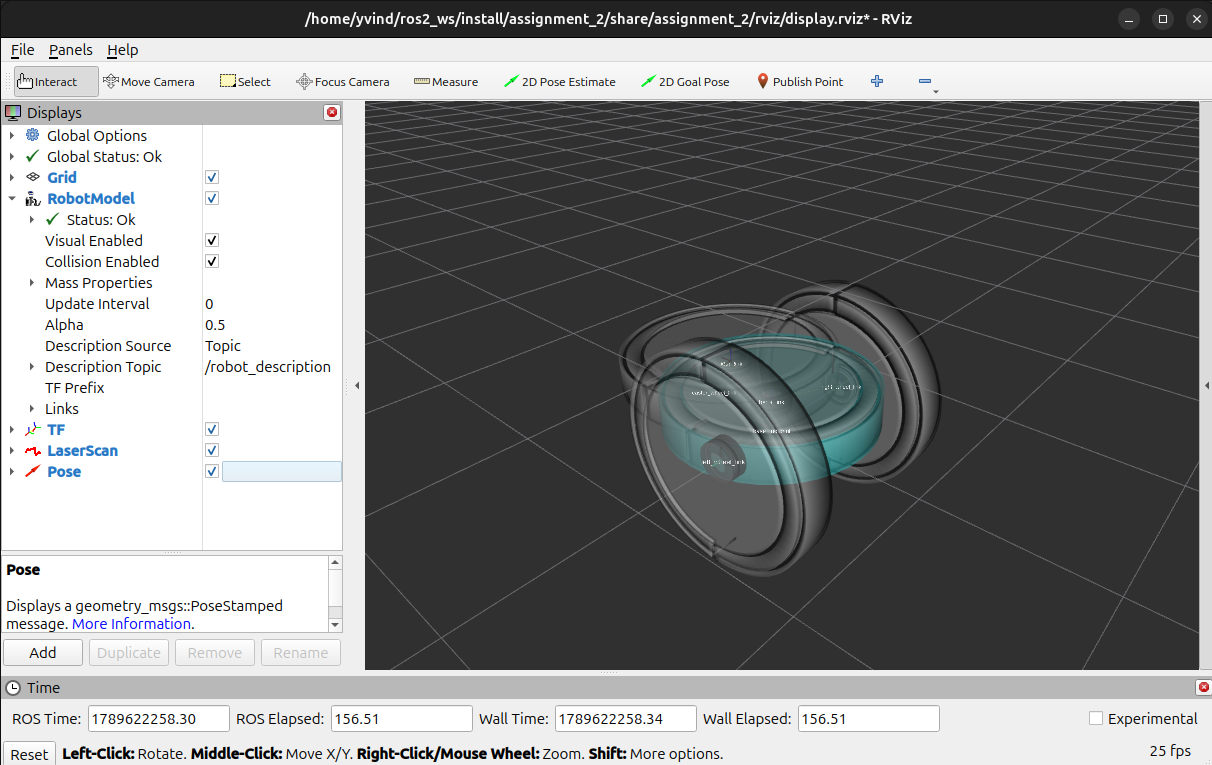
\includegraphics[width=0.7\linewidth]{mesh_overlap_error.png}
    \caption{Overlapping mesh components in RViz on the first day.}
    \label{fig:mesh_overlap_error}
\end{figure}

On the second day, the mesh references were changed back to the provided DAE files. During testing, the launch command failed because ROS could not find \texttt{assignment\_2}, even though the package had been built. This was a separate package discovery problem. Adding the package's install directory to \texttt{AMENT\_PREFIX\_PATH} allowed the model to open in RViz in the current terminal session.

The resulting model is shown in Figure~\ref{fig:doomba_meshes}. The final Xacro files reference the DAE files for the body, wheels and LiDAR.

\begin{figure}[H]
    \centering
    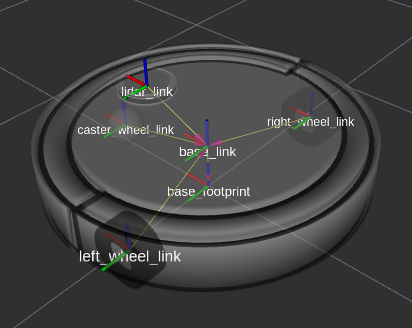
\includegraphics[width=0.75\linewidth]{doomba_rviz.png}
    \caption{The model displayed in RViz after switching back to DAE files and fixing the package discovery problem.}
    \label{fig:doomba_meshes}
\end{figure}


\subsubsection*{Physical Properties}

The dimensions, positions and masses were set according to the diagram and tables in the assignment. The values are defined as Xacro properties and reused throughout the model, with dependent dimensions calculated from these properties.


For example, the height of the body centre above the ground is:
\[
z_{\mathrm{base}} = r_{\mathrm{caster}} + \frac{h_{\mathrm{body}}}{2}
= 0.02 + \frac{0.06}{2} = 0.05~\mathrm{m}.
\]
This avoids repeating fixed values and keeps the model consistent when dimensions are changed.




\subsubsection*{Inertia Calculations}

The inertia of each part was calculated from its collision
shape, assuming uniform mass distribution. All inertias were
calculated about each part's centre of mass, with all
off-diagonal terms set to zero.

\paragraph{Body}
For the cylindrical body, $m=5.0$~kg, $r=0.16$~m and
$h=0.06$~m:
\[
I_{xx}=I_{yy}
=\frac{m}{12}(3r^2+h^2)
=\frac{5.0}{12}\left(3(0.16)^2+(0.06)^2\right)
=0.0335~\mathrm{kg\,m^2},
\]
\[
I_{zz}=\frac{1}{2}mr^2
=\frac{1}{2}(5.0)(0.16)^2
=0.0640~\mathrm{kg\,m^2}.
\]

\paragraph{Left and right wheels}
Each wheel is a cylinder with $m=0.2$~kg, $r=0.03$~m
and width $h=0.025$~m:
\[
I_{\mathrm{spin}}=\frac{1}{2}mr^2
=\frac{1}{2}(0.2)(0.03)^2
=9.00\times10^{-5}~\mathrm{kg\,m^2},
\]
\[
I_{\mathrm{other}}=\frac{m}{12}(3r^2+h^2)
=\frac{0.2}{12}\left(3(0.03)^2+(0.025)^2\right)
\approx5.54\times10^{-5}~\mathrm{kg\,m^2}.
\]
The wheels rotate about the wheel link's $y$-axis.
The inertial frame was rotated by $-\pi/2$ about $x$,
aligning the cylinder's spin axis with this direction.
Thus, in the wheel link frame, $I_{yy}=I_{\mathrm{spin}}$
and $I_{xx}=I_{zz}=I_{\mathrm{other}}$.

\paragraph{Caster}
For the spherical caster, $m=0.1$~kg and $r=0.02$~m:
\[
I_{xx}=I_{yy}=I_{zz}
=\frac{2}{5}mr^2
=\frac{2}{5}(0.1)(0.02)^2
=1.60\times10^{-5}~\mathrm{kg\,m^2}.
\]

\paragraph{LiDAR}
For the cylindrical LiDAR, $m=0.1$~kg, $r=0.03$~m
and $h=0.01$~m:
\[
I_{xx}=I_{yy}
=\frac{m}{12}(3r^2+h^2)
=\frac{0.1}{12}\left(3(0.03)^2+(0.01)^2\right)
\approx2.33\times10^{-5}~\mathrm{kg\,m^2},
\]
\[
I_{zz}=\frac{1}{2}mr^2
=\frac{1}{2}(0.1)(0.03)^2
=4.50\times10^{-5}~\mathrm{kg\,m^2}.
\]

The Xacro macros generate the corresponding
\texttt{<inertia>} elements using these formulas.
The virtual \texttt{base\_footprint} link has no mass
and therefore requires no inertia.


\subsubsection*{Diff-Drive Parameters}

The physical dimensions were defined as Xacro properties in
\texttt{robot.urdf.xacro}. The wheel radius was set to
$0.03$~m and the lateral wheel offset was set to $0.13$~m.

In \texttt{gazebo\_control.xacro}, the Gazebo diff-drive plugin
uses these properties directly:

\begin{verbatim}
<wheel_separation>${2*wheel_offset_y}</wheel_separation>
<wheel_radius>${wheel_radius}</wheel_radius>
\end{verbatim}



\subsubsection*{Collision Model Verification}

The model was rebuilt and opened in RViz. The collision
model was inspected with both \texttt{Visual Enabled}
and \texttt{Collision Enabled} selected. Alpha was set
to 0.5 so the collision shapes could be seen together
with the meshes. The shapes appeared consistent with
the size and position of the corresponding robot parts.

\begin{figure}[H]
    \centering
    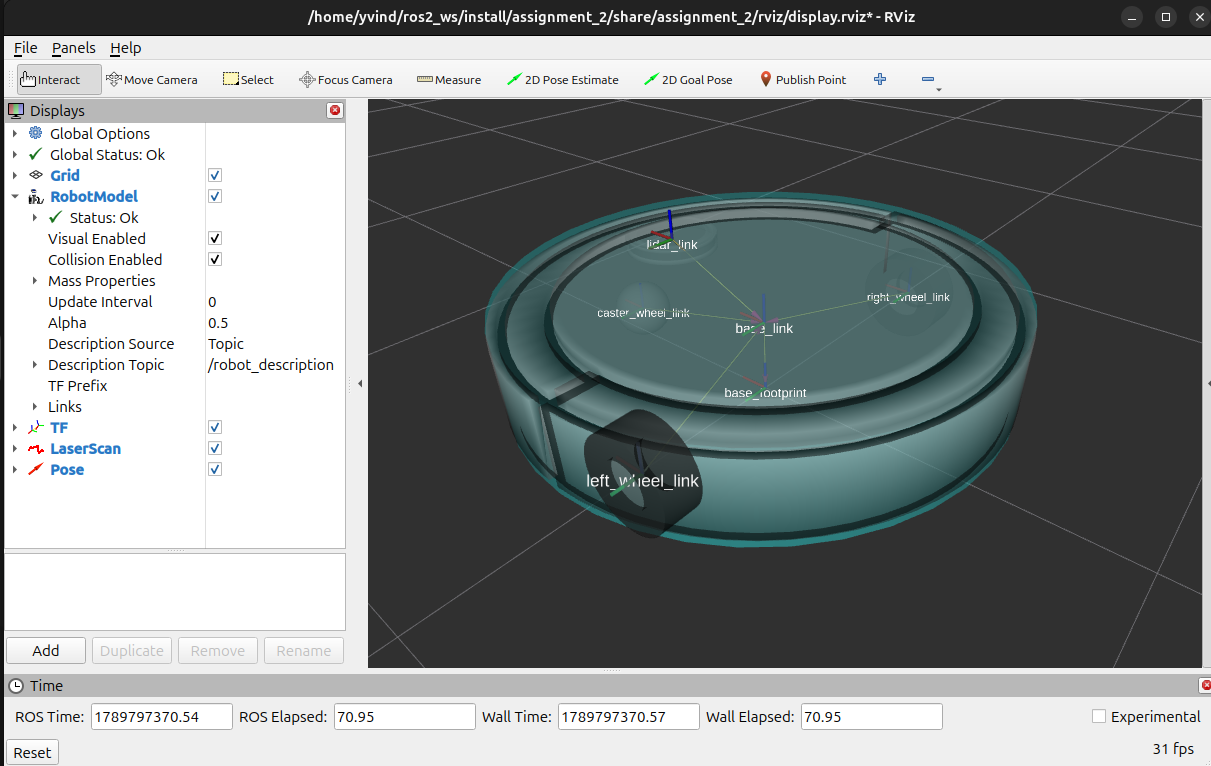
\includegraphics[width=0.9\linewidth]{collision_overlay.png}
    \caption{Visual meshes and collision shapes displayed
    together in RViz with Alpha set to 0.5.}
    \label{fig:collision_overlay}
\end{figure}



\subsubsection*{Frame Verification}

With the model running, \texttt{tf2\_echo} was used to check
the positions of the LiDAR and left wheel relative to
\texttt{base\_link}. The translations were
$[0.080,\ 0.000,\ 0.035]$~m for the LiDAR and
$[-0.030,\ 0.130,\ -0.020]$~m for the left wheel.
Both matched the joint origins in the assignment
to the nearest millimetre.

\begin{figure}[H]
    \centering
    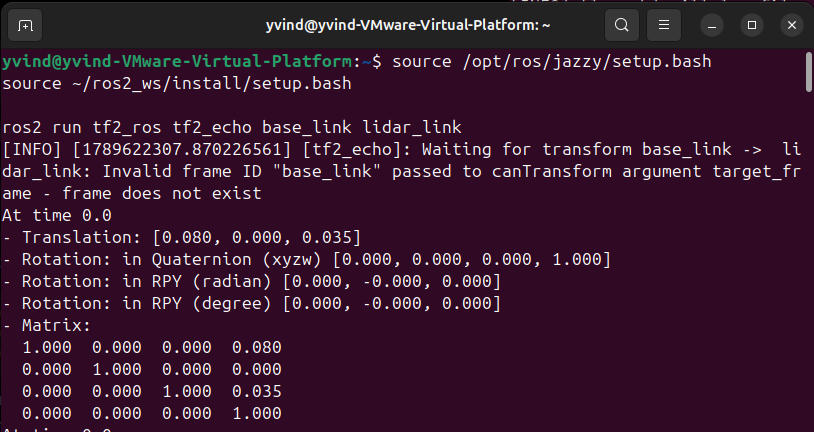
\includegraphics[width=0.85\linewidth]{tf_lidar.png}

    \vspace{0.3cm}
    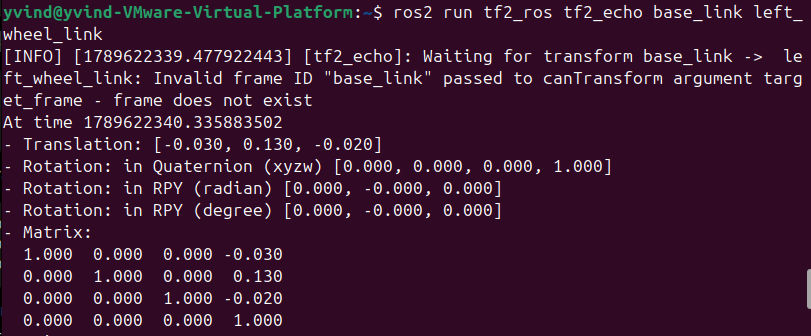
\includegraphics[width=0.85\linewidth]{tf_left_wheel.png}
    \caption{Transforms from base\_link to lidar\_link
    (top) and left\_wheel\_link (bottom).}
    \label{fig:tf_verification}
\end{figure}

\FloatBarrier
\section{Task 2: The Maze Challenge}


\FloatBarrier
\section{Task 3: Make the Node Adaptive and Configurable}


\FloatBarrier
\section{Task 4: Where Does the Robot Think It Is?}


\FloatBarrier
\section{Problems Encountered and Solutions}


\section{Reflection}


\section{Use of AI}


\end{document}